\section{Extended partitioning: Add partition}
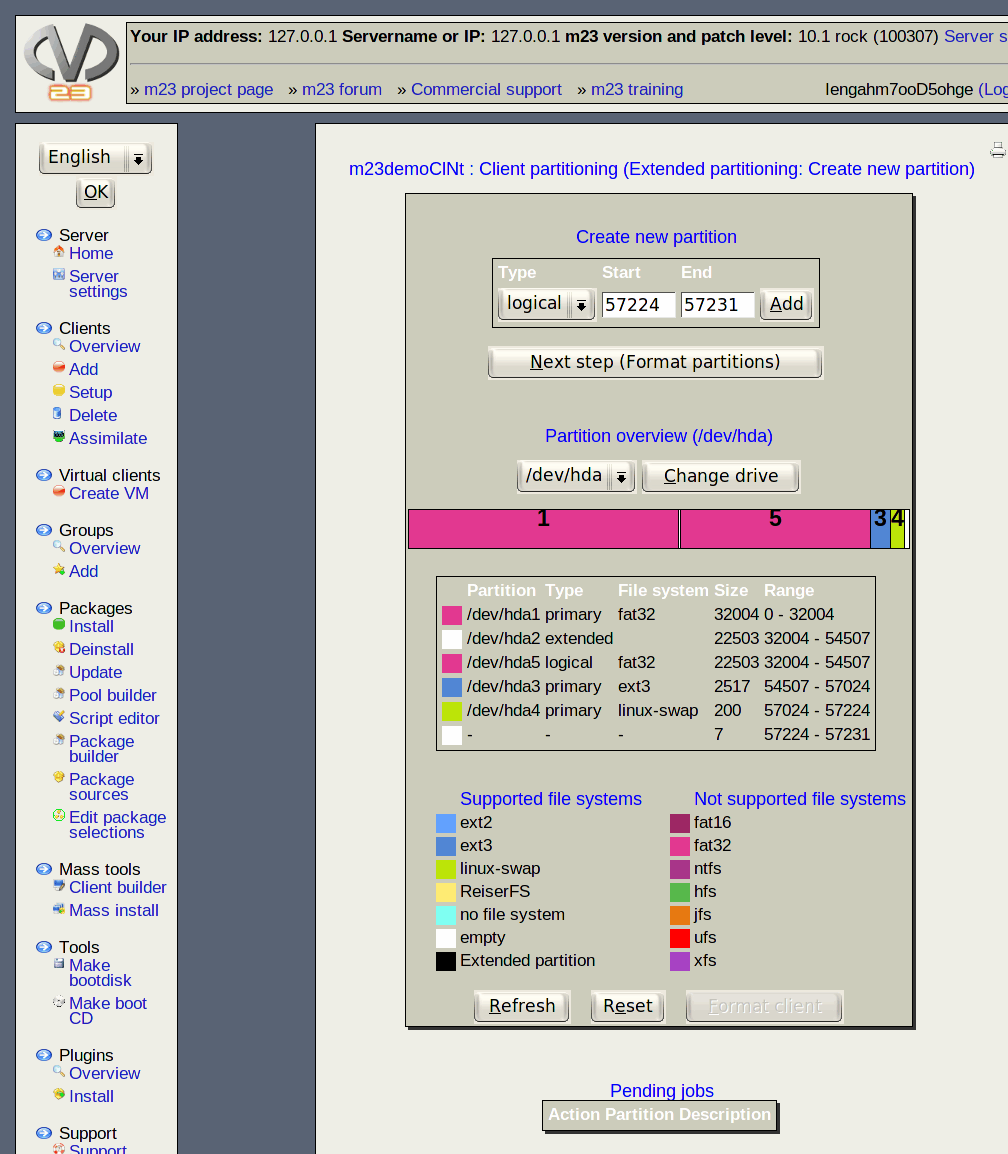
\includegraphics[scale=0.4]{/mdk/doc/manual/screenshots/en/fdisk-extended1.png} \\
\begin{itemize}
\item You can add new partitions now. Select if you want to create a primary, extended or logical partition. Enter the start and end position of your new partition and click on \textit{"Add"}. You can find some information about the partition types at the bottom of the page.\\
\item \textit{"Partition overview"} shows you free spaces which can be used for the creation of new partitions. Free spaces are colored white. Have a look at the ranges at the \textit{"Range"} column to check where you can add new partitions.\\
\item If there is not enough space to create a new partition, go back with the \textit{"Back"} button of your browser until you see the "delete partitions" dialog.\\
\item Go to the next step \textit{""}, when you have created all necessary partitions.\\
\end{itemize}
\subsection{Information: Partition types}
\begin{itemize}
 \item \textbf{primary:} You can create a maximum amount of 4 primary partitions.\\
 \item \textbf{extended:} An extended partition is a special type of a primary partition. You can only create one extended partition. Within an extended partition you can create logical partitions.\\
 \item \textbf{logical:} Logical partitions can be created within an extended partition only. Logical partitions are a simple way to create more then 4 partitions. Don't forget to create an extended partition first.\\
\end{itemize}
